 \documentclass[11pt,a4paper]{article}
\usepackage[utf8]{inputenc}		% LaTeX, comprend les accents !
\usepackage[T1]{fontenc}
\usepackage{natbib}	
%\usepackage[square,sort&compress,sectionbib]{natbib}		% Doit être chargé avant babel      
\usepackage[frenchb,english]{babel}
\usepackage{lmodern}
\usepackage{amsmath,amssymb, amsthm}
\usepackage{a4wide}
\usepackage[capposition=top]{floatrow}
\usepackage{verbatim}
\usepackage{float}
\usepackage{placeins}
\usepackage{flafter}
\usepackage{longtable}
\usepackage{import}
\usepackage{pdflscape}
\usepackage{rotating}
\usepackage{hhline}
\usepackage{multirow}
\usepackage{booktabs}
\usepackage[pdftex,pdfborder={0 0 0},colorlinks=true,linkcolor=blue,urlcolor=blue,citecolor=blue,bookmarksopen=true]{hyperref}
\usepackage{eurosym}
%\usepackage{breakcites}
\usepackage[autostyle]{csquotes}
%\usepackage{datetime}
\usepackage{natbib}
\usepackage{setspace}
\usepackage{lscape}
\usepackage[usenames]{color}
\usepackage{indentfirst}
\usepackage{url}
\usepackage{enumitem}
\usepackage{multirow}
\usepackage{subcaption}
\usepackage[justification=centering]{caption}
\bibliographystyle{agsm}

\usepackage{array}

\newcommand{\isEmbedded}{true}

\graphicspath{{Figures/}}


\begin{document}

\selectlanguage{frenchb}
\title{Analyse des trajectoires dans les grilles \\ Focus sur les adjoints techniques}


\author{Simon Rabat\'e et Mahdi Ben Jelloul}


\maketitle

% Introduction
Ce note propose une première analyse des trajectoires indiciaires sur un sous-échantillon de la base carrière: les individus qui se trouvent dans le corps des adjoints techniques pour toutes les années entre 2007 et 2015. 



% Section I: Analyse des grilles
\section{Le corps des adjoints techniques}

Le corps des adjoints techniques comporte quatre grades distincts: les adjoints technique de 2eme classe, les adjoints techniques de 1ere classe, les adjoints techniques principal de 2e classe et les adjoints technique principal de 1ere classe. 

Dans la suite de la note nous utilisons les abréviations suivantes pour ces différents grades: AT2, AT1, ATP2 et ATP1 respectivement. 

Le tableau ci-dessous précise les conditions de passage au grade immédiatement supérieur\footnote{Source: \url{http://www.cdg45.fr/racine/accueil/gestion_des_ressources_humaines/cadres_d_emplois_de_la_fpt/filiere_technique/adjoint_technique_territorial/avancement_de_grade/avancement_de_grade}.}. 



\begin{table}[h!]
\label{means}
\centering
\caption{Conditions d'avancement pour le corps des AT} 
\begin{tabular}{l|c|ccc}
\toprule
 Grade  & Type d'avancement&  \multicolumn{3}{c}{|||| Condition de ... ||||}  \\
		&  				   &  Durée dans le grade	&  Échelon	dans le grade & Durée dans l'échelon \\
\midrule
AT2  &	Avec exam pro. 	&   3 ans  & 	4  & NA \\
AT2  &	Sans exam pro. 	& 	10 ans &	7  &	NA \\
AT1  & Tous				& 	6 ans  &	5  &	NA \\
ATP2 & Tous				& 	5 ans  &	6  &	2 ans  \\	
%	
\bottomrule
\end{tabular}
\end{table}


Les grilles de ces différents grades ont connu de nombreuses évolutions dans les années considérées (4 pour les trois premiers, 6 pour le grade ATP1). Les graphiques \ref{echelon_by_neg} et \ref{echelon_by_date} proposent une visualisation de ces différentes grilles. 



\begin{figure}[ht] 
  \caption{Evolution des grilles: grade par grade}
  \label{echelon_by_neg} 
  \begin{subfigure}[b]{0.55\linewidth}
      \caption{Grade AT2} 
    \label{echelon_by_neg_0} 
    \centering
    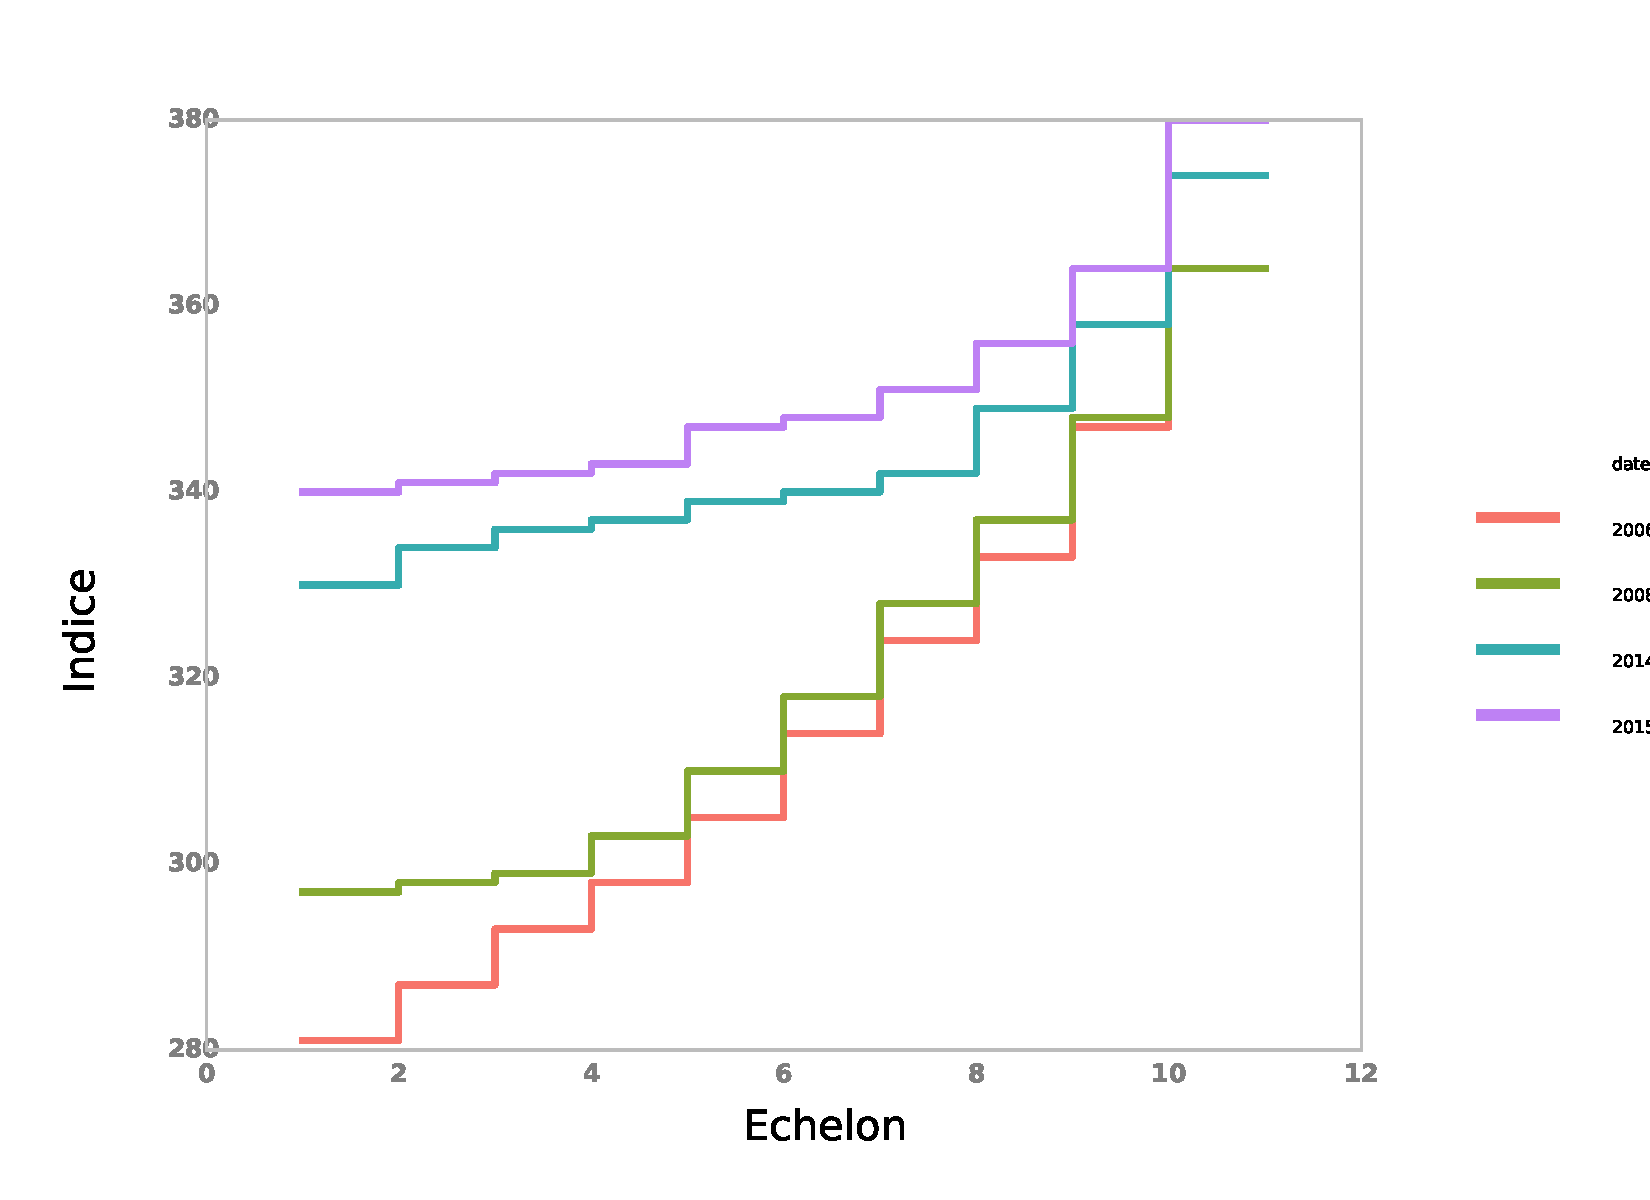
\includegraphics[width=1\linewidth]{0_grille_by_neg.pdf} 
    \vspace{4ex}
  \end{subfigure}%% 
  \begin{subfigure}[b]{0.55\linewidth}
        \caption{Grade AT1} 
    \label{echelon_by_neg_1} 
    \centering
    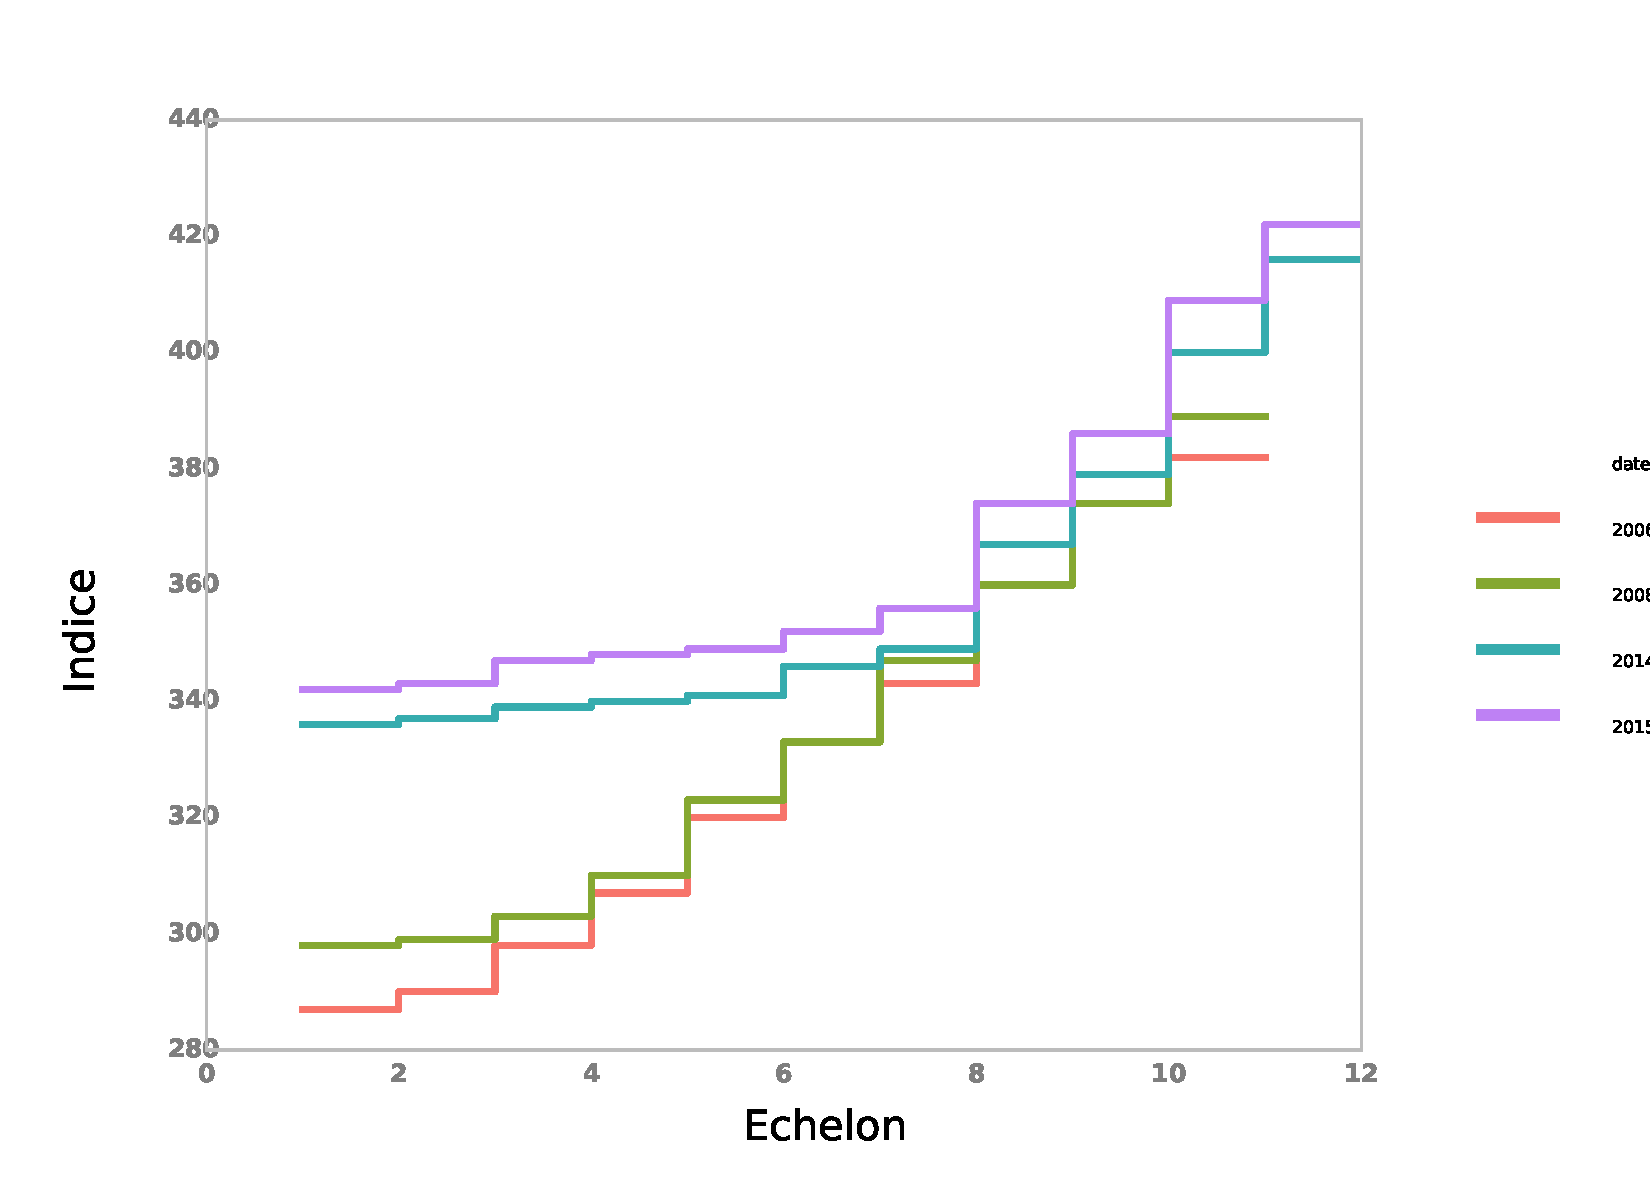
\includegraphics[width=1\linewidth]{1_grille_by_neg.pdf} 
    \vspace{4ex}
  \end{subfigure} 
  \begin{subfigure}[b]{0.55\linewidth}
        \caption{Grade ATP2} 
    \label{echelon_by_neg_2} 
    \centering
    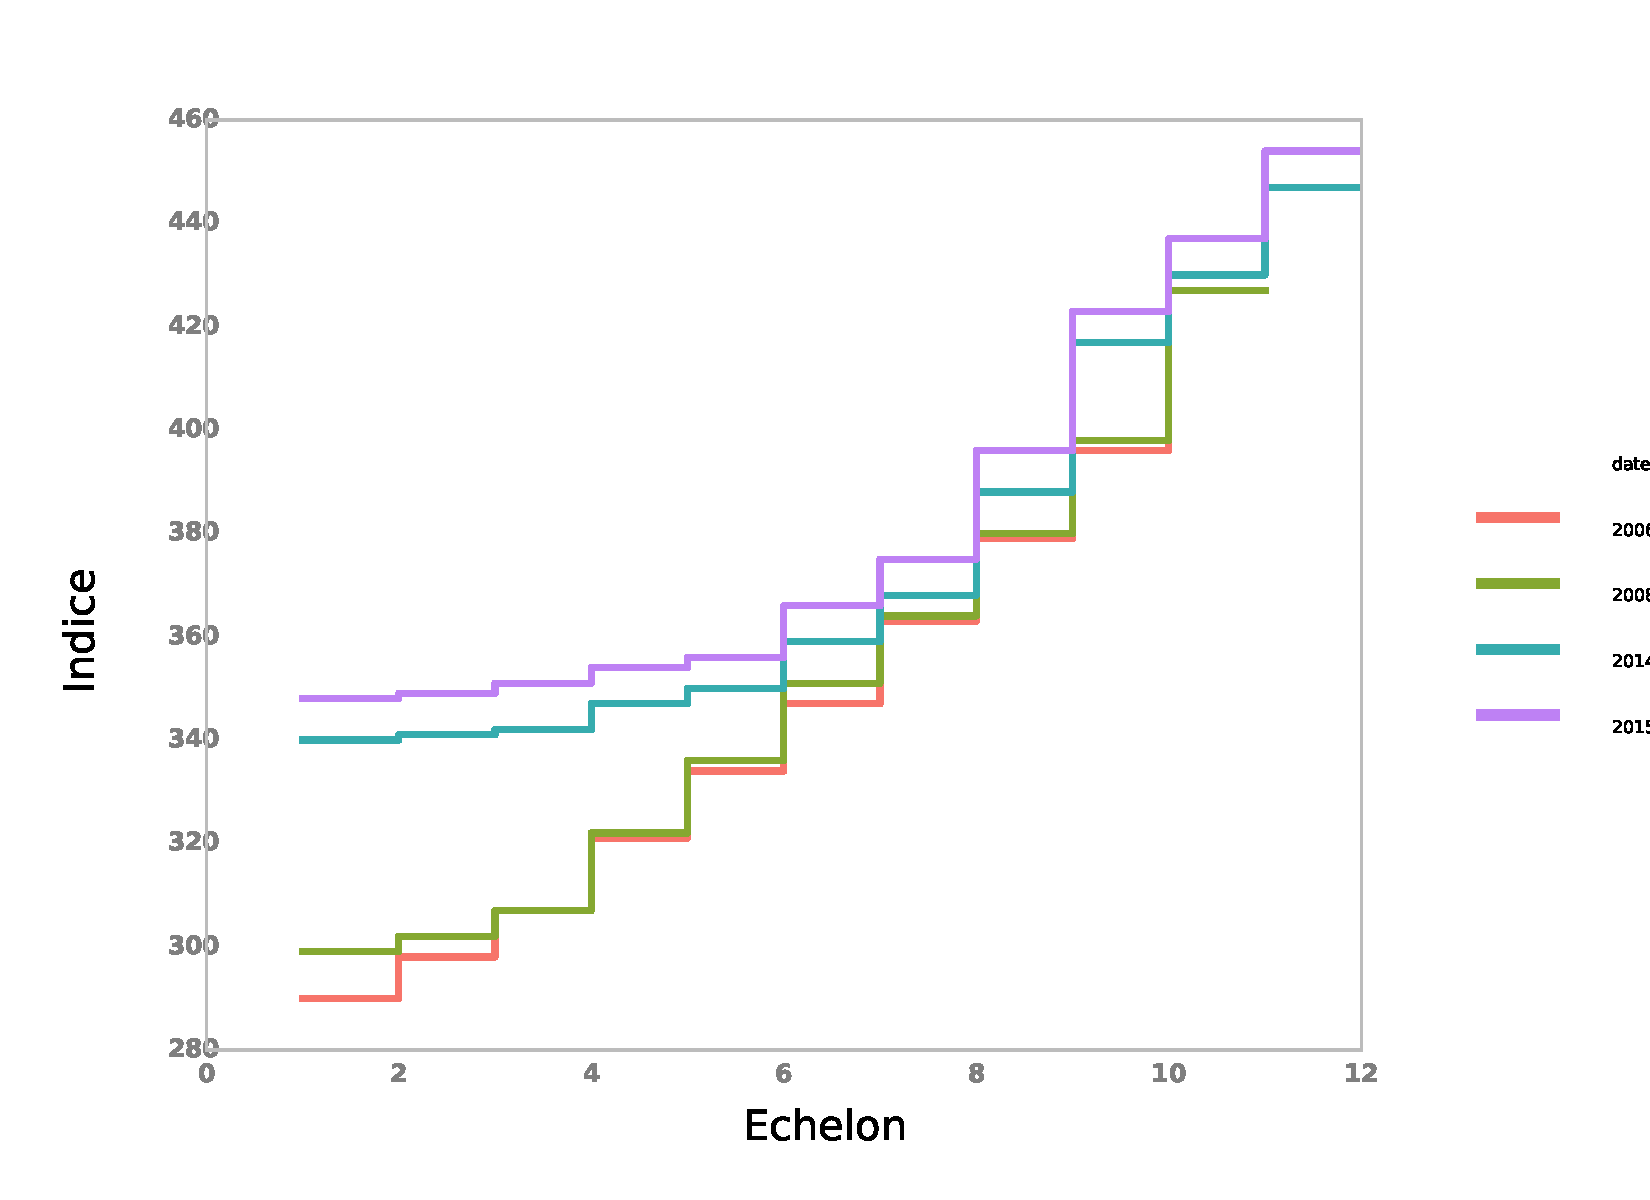
\includegraphics[width=1\linewidth]{2_grille_by_neg.pdf} 
  \end{subfigure}%%
  \begin{subfigure}[b]{0.55\linewidth}
        \caption{Grade ATP1} 
    \label{echelon_by_neg_3} 
    \centering
    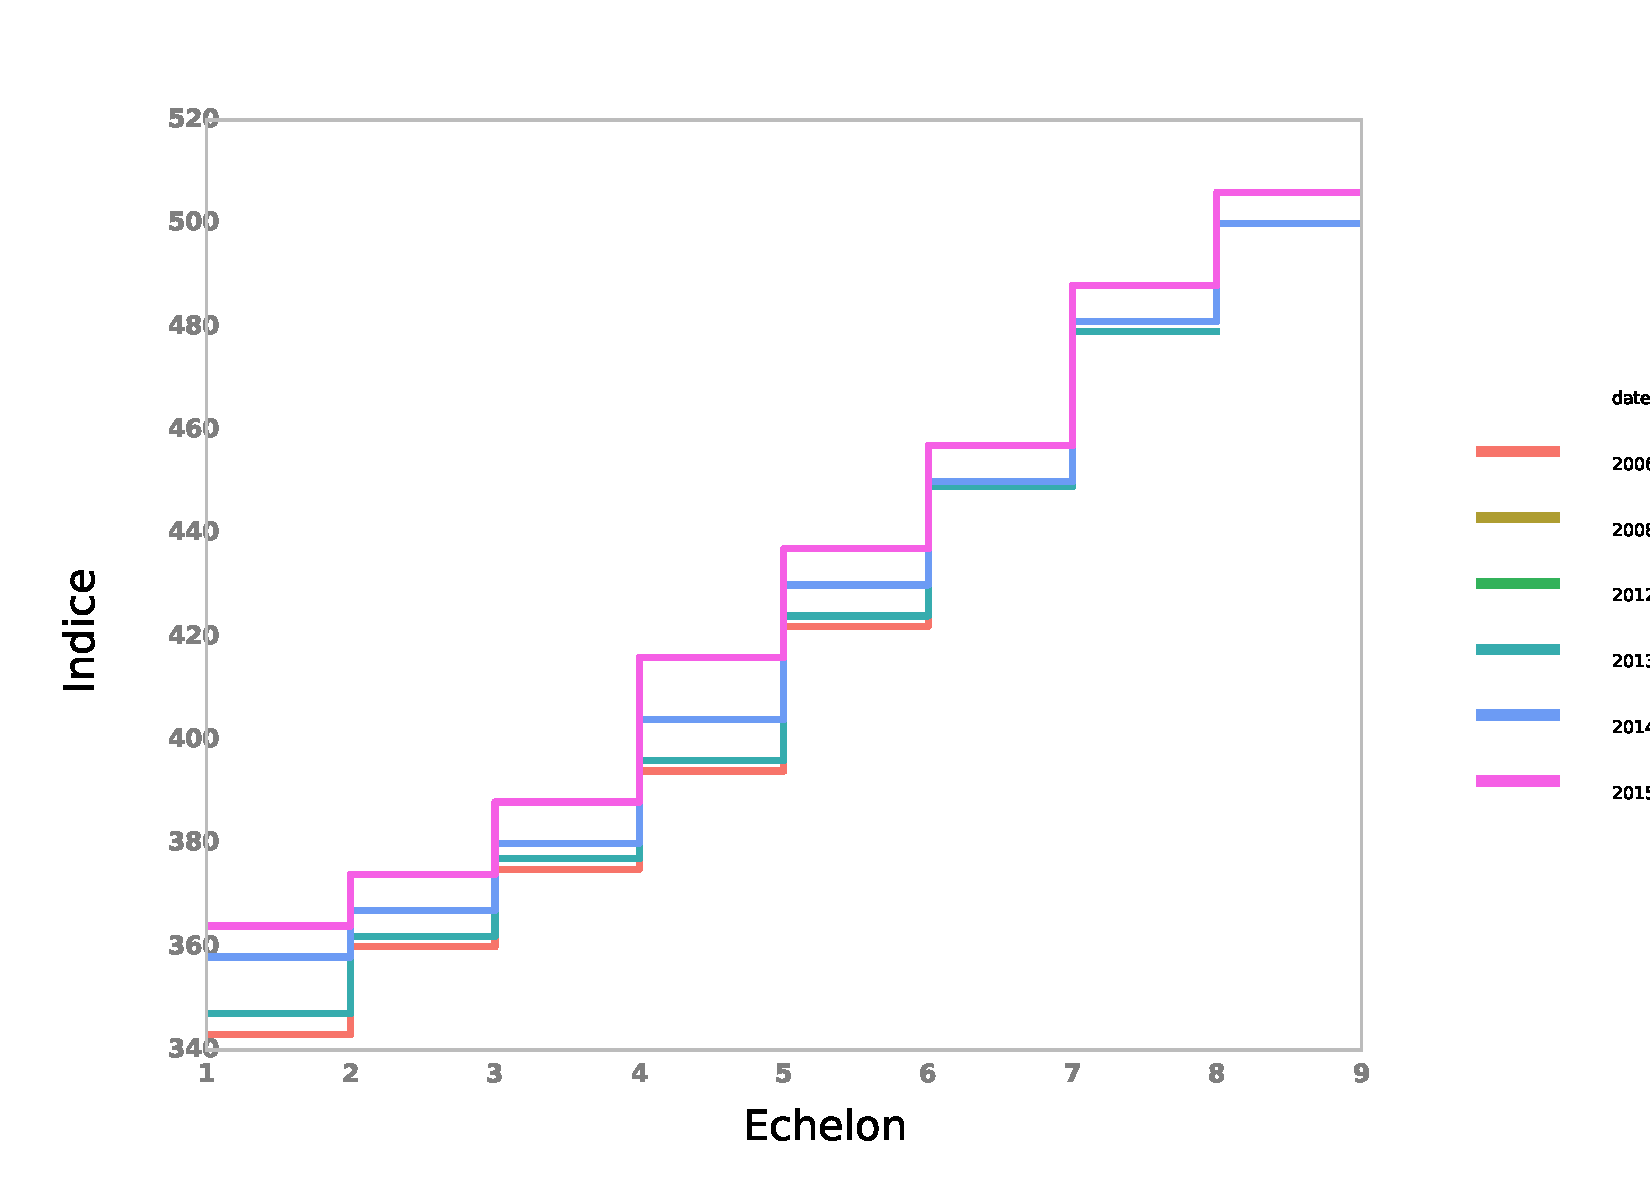
\includegraphics[width=1\linewidth]{3_grille_by_neg.pdf} 
  \end{subfigure} 
\end{figure}




\begin{figure}[ht] 
  \caption{Évolution des grilles: niveau relatif des grades}
  \label{echelon_by_date} 
  \begin{subfigure}[b]{0.55\linewidth}
      \caption{Année 2006} 
    \label{echelon_by_neg_0} 
    \centering
    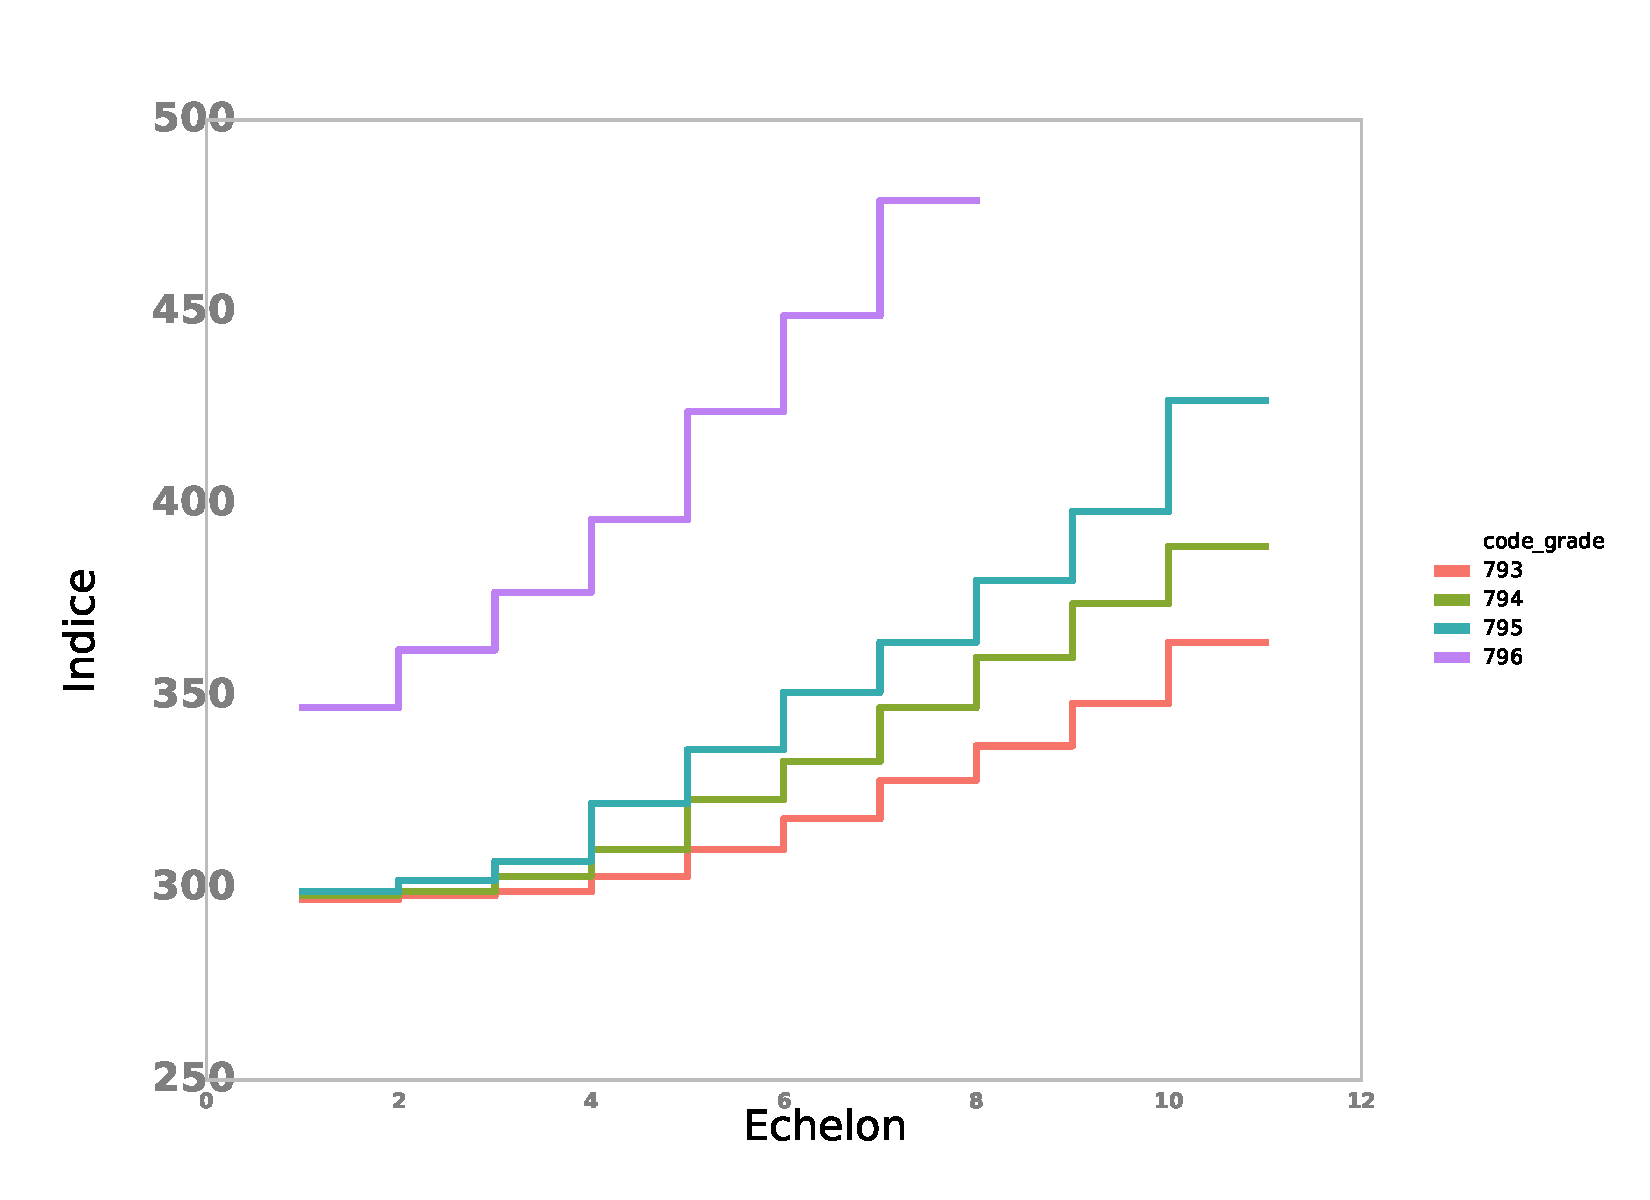
\includegraphics[width=1\linewidth]{0_grille_by_date.pdf} 
    \vspace{4ex}
  \end{subfigure}%% 
  \begin{subfigure}[b]{0.55\linewidth}
      \caption{Année 2008} 
    \label{echelon_by_neg_1} 
    \centering
    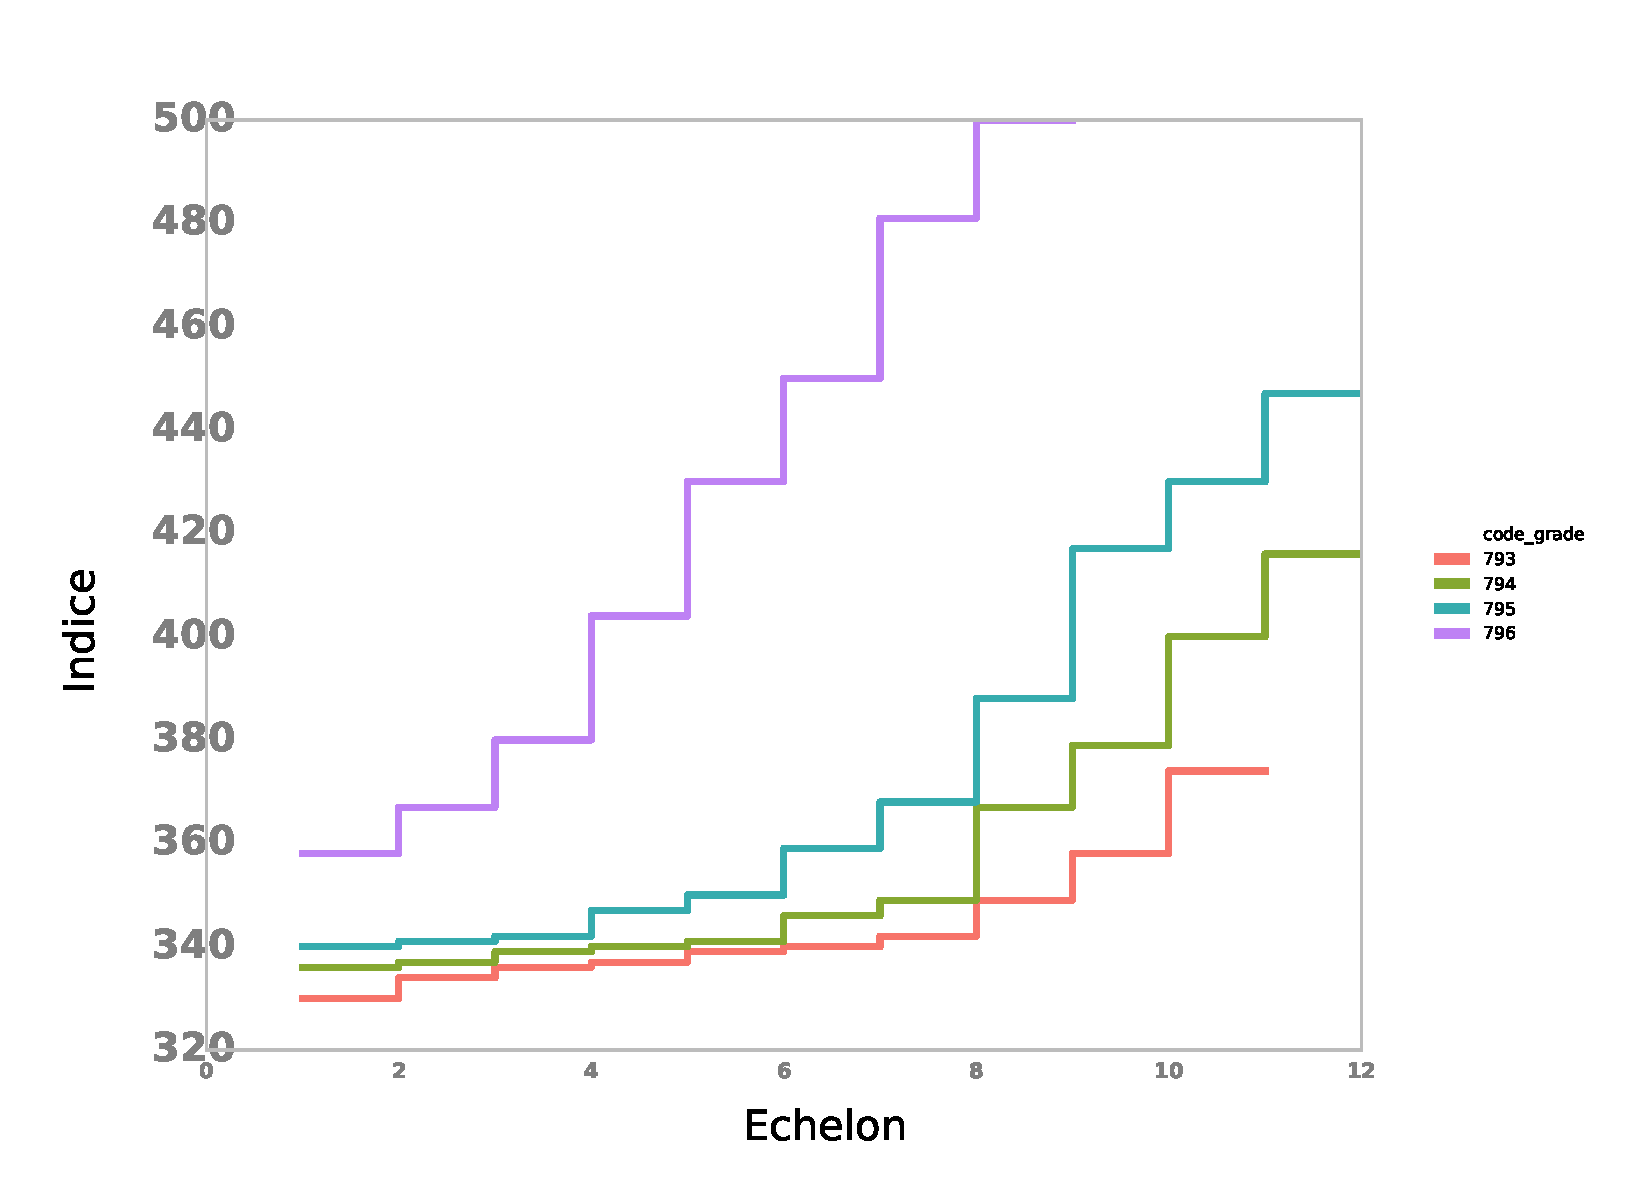
\includegraphics[width=1\linewidth]{1_grille_by_date.pdf} 
    \vspace{4ex}
  \end{subfigure} 
  \begin{subfigure}[b]{0.55\linewidth}
      \caption{Année 2014} 
    \label{echelon_by_neg_2} 
    \centering
    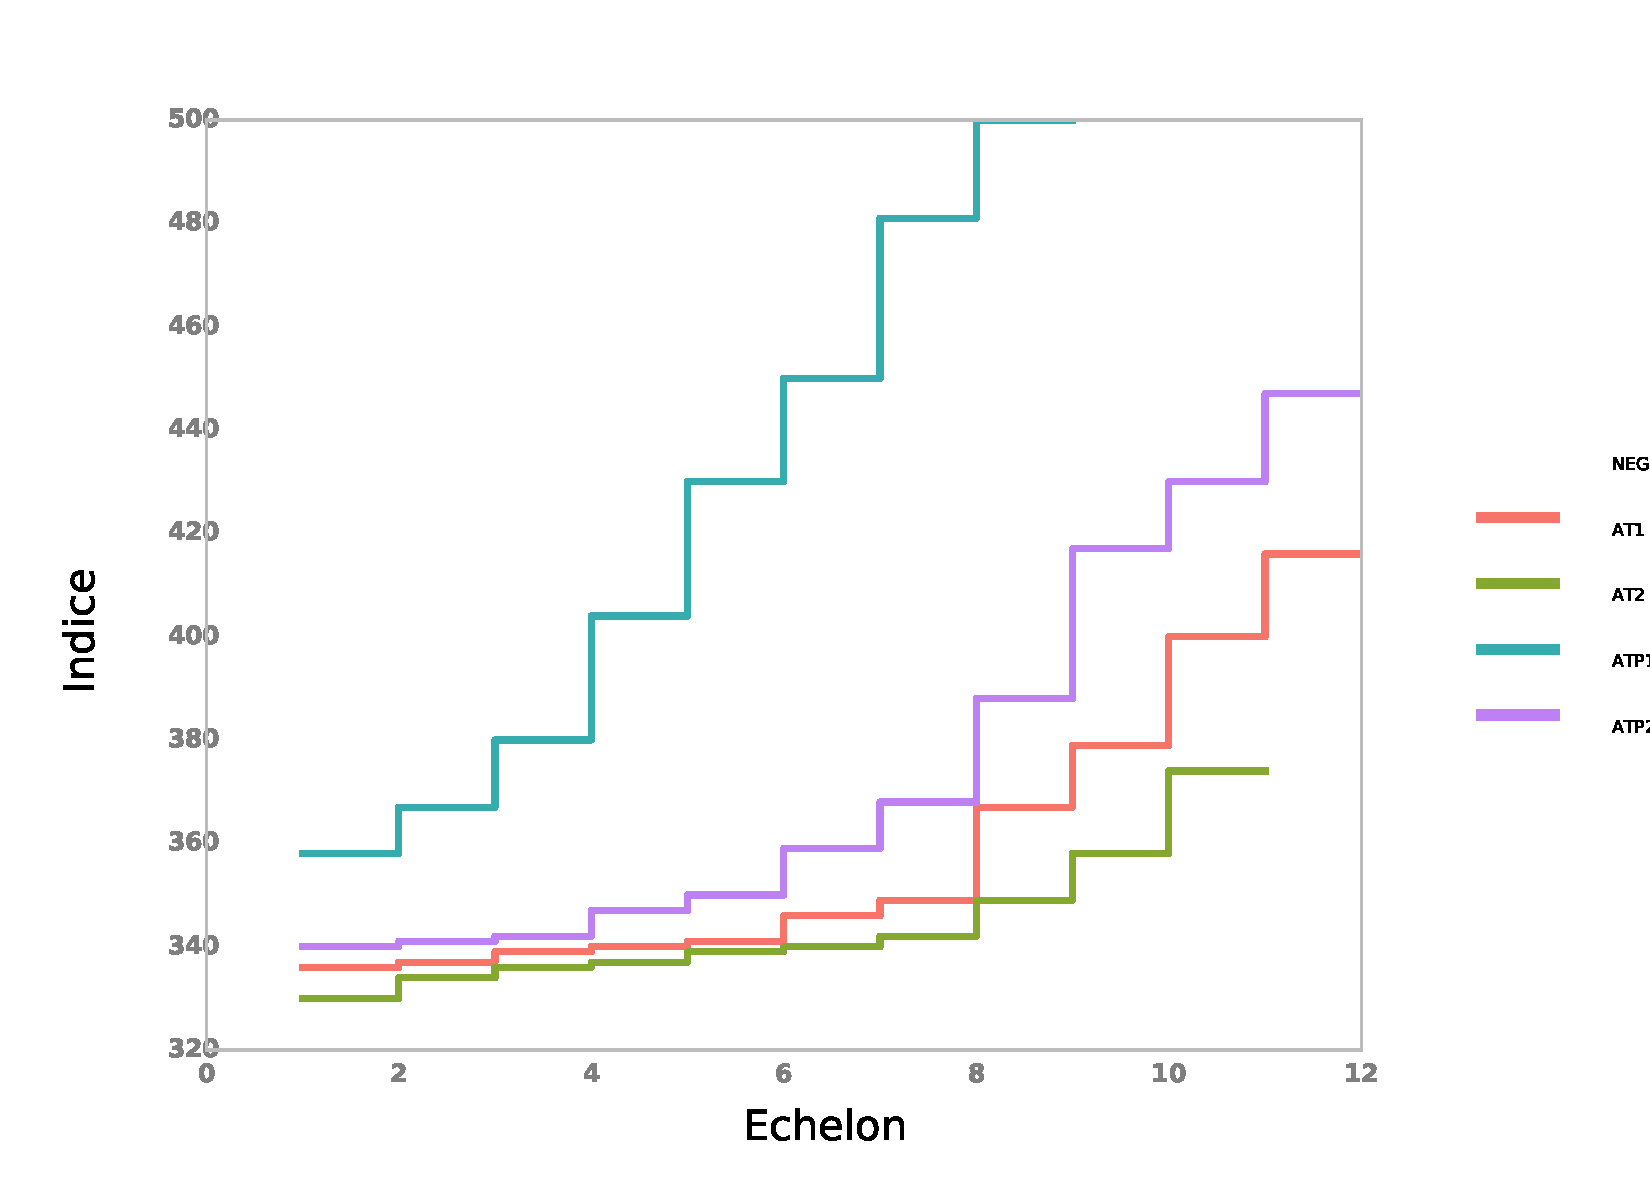
\includegraphics[width=1\linewidth]{2_grille_by_date.pdf} 
  \end{subfigure}%%
  \begin{subfigure}[b]{0.55\linewidth}
      \caption{Année 2015} 
    \label{echelon_by_neg_3} 
    \centering
    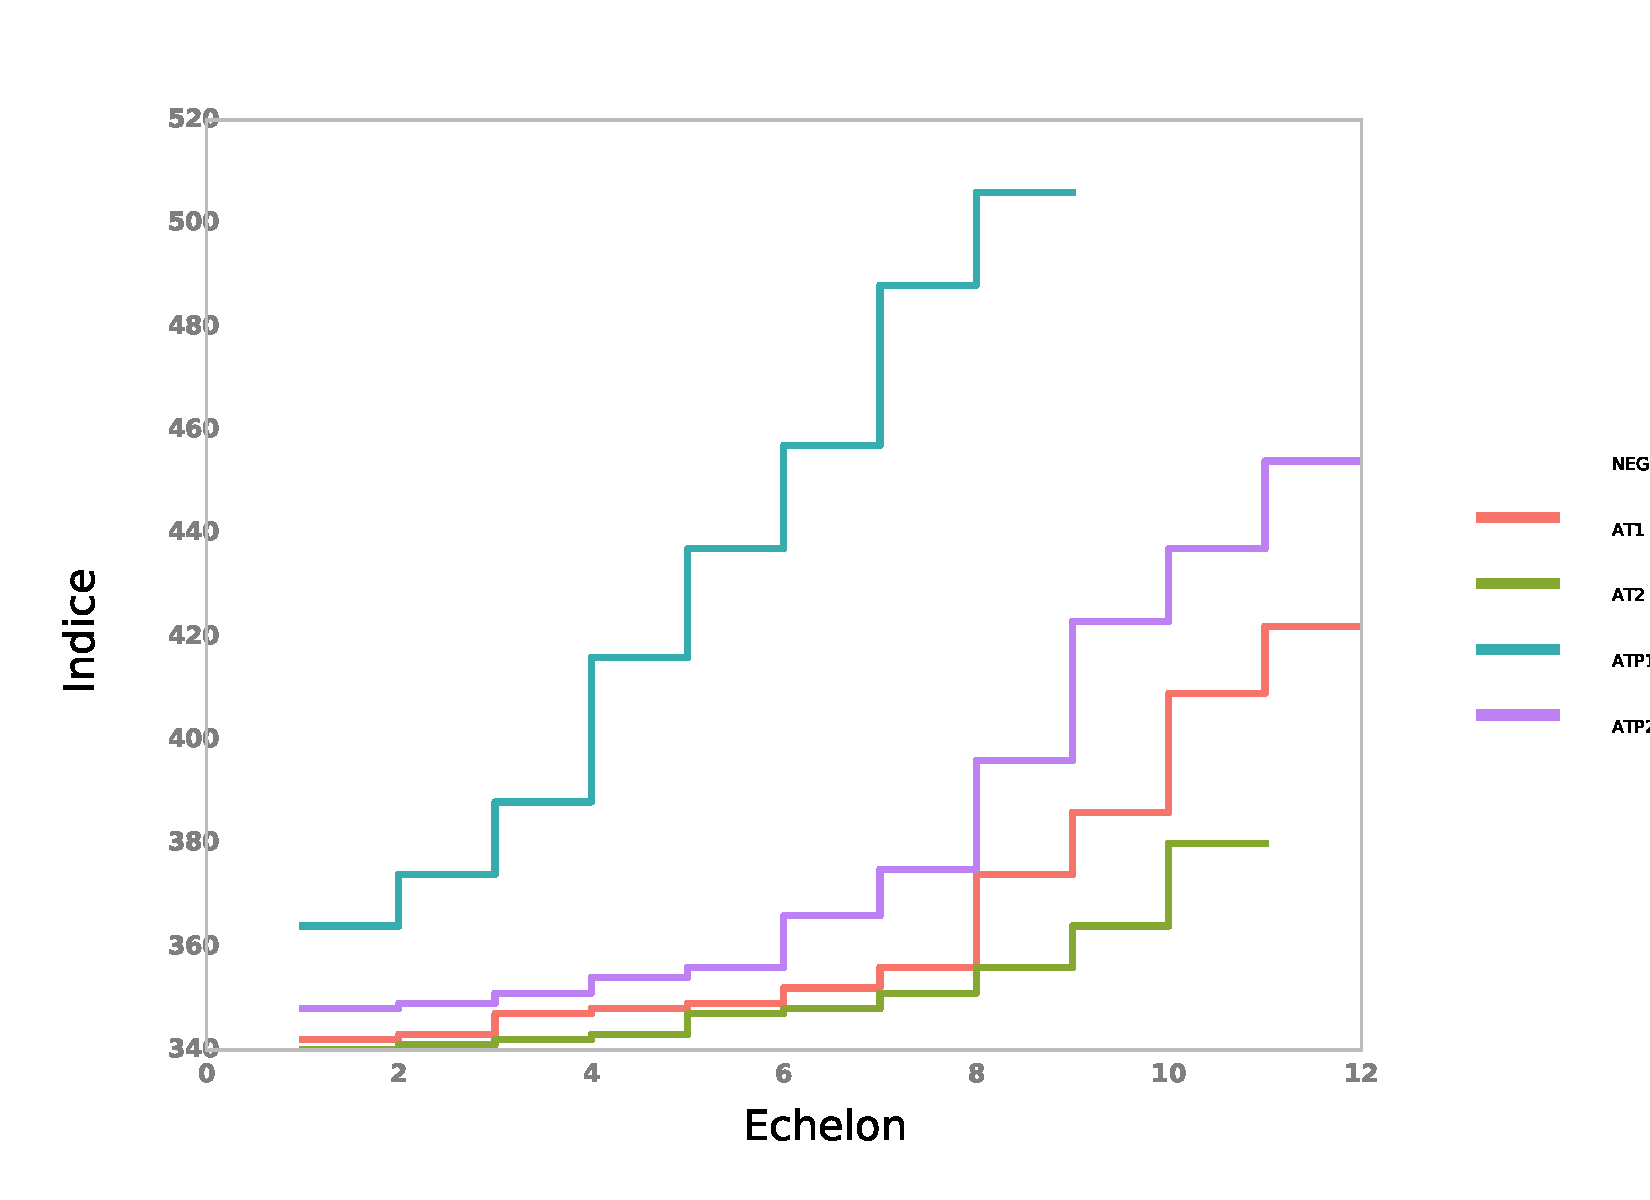
\includegraphics[width=1\linewidth]{3_grille_by_date.pdf} 
  \end{subfigure} 
\end{figure}




\clearpage


Questions et pistes amelioration pour améliorer la base: 
\begin{itemize}
\item Correction du neg à partir de l'indice. 
\item Echelon = - 1?
\end{itemize}


% Section II: Travail sur les données
\section{Travail sur les données}

\subsection{Sélection d'une sous-population}


\subsection{Imputation d'une durée initiale dans le grade}


% Section III: Statistiques descriptives
\section{Statistiques descriptives}




\end{document}


